\documentclass[10pt,a4paper]{article}
\usepackage[UTF8,fontset = windows]{ctex}
\setCJKmainfont[BoldFont=黑体,ItalicFont=楷体]{华文中宋}
\usepackage{amssymb,amsmath,amsfonts,amsthm,mathrsfs,dsfont,graphicx}
\usepackage{ifthen,indentfirst,enumerate,color,titletoc}
\usepackage{tikz}
\usepackage{multicol}
\usepackage{makecell}
\usepackage{longtable}
\usetikzlibrary{arrows,calc,intersections,patterns,decorations.pathreplacing,3d,angles,quotes}
\usepackage[bf,small,indentafter,pagestyles]{titlesec}
\usepackage[top=1in, bottom=1in,left=0.8in,right=0.8in]{geometry}
\renewcommand{\baselinestretch}{1.65}
\newtheorem{defi}{定义~}
\newtheorem{eg}{例~}
\newtheorem{ex}{~}
\newtheorem{rem}{注~}
\newtheorem{thm}{定理~}
\newtheorem{coro}{推论~}
\newtheorem{axiom}{公理~}
\newtheorem{prop}{性质~}
\newcommand{\blank}[1]{\underline{\hbox to #1pt{}}}
\newcommand{\bracket}[1]{(\hbox to #1pt{})}
\newcommand{\onech}[4]{\par\begin{tabular}{p{.9\textwidth}}
A.~#1\\
B.~#2\\
C.~#3\\
D.~#4
\end{tabular}}
\newcommand{\twoch}[4]{\par\begin{tabular}{p{.46\textwidth}p{.46\textwidth}}
A.~#1& B.~#2\\
C.~#3& D.~#4
\end{tabular}}
\newcommand{\vartwoch}[4]{\par\begin{tabular}{p{.46\textwidth}p{.46\textwidth}}
(1)~#1& (2)~#2\\
(3)~#3& (4)~#4
\end{tabular}}
\newcommand{\fourch}[4]{\par\begin{tabular}{p{.23\textwidth}p{.23\textwidth}p{.23\textwidth}p{.23\textwidth}}
A.~#1 &B.~#2& C.~#3& D.~#4
\end{tabular}}
\newcommand{\varfourch}[4]{\par\begin{tabular}{p{.23\textwidth}p{.23\textwidth}p{.23\textwidth}p{.23\textwidth}}
(1)~#1 &(2)~#2& (3)~#3& (4)~#4
\end{tabular}}
\begin{document}

\begin{enumerate}[1.]
\item 已知$z=1+\mathrm{i}$(其中$\mathrm{i}$为虚数单位), 则$2\overline{z}=$\blank{50}.
\item 双曲线$\dfrac{x^2}{9}-y^2=1$的实轴长为\blank{50}.
\item 函数$f(x)=\cos^2 x-\sin ^2 x+1$的周期为\blank{50}.
\item 已知$a$是实数, 行列式$\begin{vmatrix}    a & 1 \\ 3 & 2\end{vmatrix}$的值与行列式$\begin{vmatrix}    a & 0 \\ 4 & 1\end{vmatrix}$的值相等, 则$a=$\blank{50}.
\item 已知圆柱的高为$4$, 底面积为$9\pi$, 则圆柱的侧面积为\blank{50}.
\item 已知$x,y$满足$\begin{cases}x+y\le 0, \\ x-y-1\le 0,\end{cases}$ 则$z=x+2y$的最小值为\blank{50}.
\item 二项式$(3+x)^n$的展开式中, $x^2$项的系数是常数项的$5$倍, 则$n=$\blank{50}.
\item 设$a$是常数, 若函数$f(x)=\begin{cases} a^2x-1, & x<0, \\ x+a, & x>0, \\ 0, & x=0 \end{cases}$为奇函数, 则$a$的值为\blank{50}.
\item 为了检查学生的身体素质指标, 从游泳类$1$项, 球类$3$项, 田径类$4$项共$8$项项目中随机抽取$4$项进行检测, 则每一类都被抽到的概率为\blank{50}.
\item 已知等差数列$\{a_n\}$的公差不为零, $S_n$为其前$n$项和, 若$S_3=0$, 则$S_i$($i=1,2,\cdots,100$)中不同的数值有\blank{50}个.
\item 若平面向量$\overrightarrow a,\overrightarrow b,\overrightarrow c$满足$|\overrightarrow a|=|\overrightarrow b|=|\overrightarrow c|=\lambda$, 且$\overrightarrow a\cdot \overrightarrow b=0$, $\overrightarrow a\cdot \overrightarrow c=2$, $\overleftrightarrow b\cdot \overrightarrow c=1$, 则$\lambda=$\blank{50}.
\item 设定义在$[0,+\infty)$上的函数$f(x)$的值域为$A_f$. 若对任意满足$f(x)=f(\dfrac 1{x+1})$的函数$f(x)$, 集合$\{y|y=f(x), \ x\in [0,a]\}$总可以取得$A_f$中的所有值, 则实数$a$的取值范围为\blank{50}.
\item 若集合$A=[-1,2)$, $B=\mathbf{Z}$, 则$A\cap B=$\bracket{20}.
\fourch{$\{-2,-1,0,1\}$}{$\{-1,0,1\}$}{$\{-1,0\}$}{$\{-1\}$}
\item 若实数$a,b$满足$a>b>0$, 下列不等式中恒成立的是\bracket{20}.
\fourch{$a+b>2\sqrt{ab}$}{$a+b<2\sqrt{ab}$}{$\dfrac a2+2b>2\sqrt{ab}$}{$\dfrac a2+2b<2\sqrt{ab}$}
\item 如图, 正方体$ABCD-A_1B_1C_1D_1$中, $P,Q,R,S$分别为棱$AB,BC,BB_1,CD$的中点, 联结$A_1S,B_1D$. 空间任意两点$M,N$, 若线段$MN$上不存在点在线段$A_1S,B_1D$上, 则称$M,N$两点可视, 则下列选项中, 与点$D_1$可视的为\bracket{20}.
\begin{center}
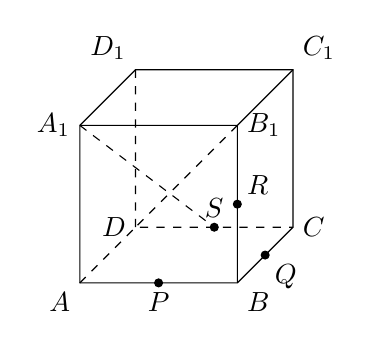
\begin{tikzpicture}[>=latex]
\draw (0,0) node [below left] {$A$} coordinate (A) --++ (2,0) node [below right] {$B$} coordinate (B) --++ (45:{2/2}) node [right] {$C$} coordinate (C)
--++ (0,2) node [above right] {$C_1$} coordinate (C1)
--++ (-2,0) node [above left] {$D_1$} coordinate (D1) --++ (225:{2/2}) node [left] {$A_1$} coordinate (A1) -- cycle;
\draw (A) ++ (2,2) node [right] {$B_1$} coordinate (B1) -- (B) (B1) --++ (45:{2/2}) (B1) --++ (-2,0);
\draw [dashed] (A) --++ (45:{2/2}) node [left] {$D$} coordinate (D) --++ (2,0) (D) --++ (0,2);
\filldraw ($(A)!0.5!(B)$) circle (0.05) node [below] {$P$};
\filldraw ($(C)!0.5!(B)$) circle (0.05) node [below right] {$Q$};
\filldraw ($(B1)!0.5!(B)$) circle (0.05) node [above right] {$R$};
\filldraw ($(C)!0.5!(D)$) circle (0.05) node [above] {$S$} coordinate (S);
\draw [dashed] (A1) -- (S) (B1) -- (D);
\end{tikzpicture}
\end{center}
\fourch{点$P$}{点$B$}{点$R$}{点$Q$}
\item 设集合$\Omega = \{(x,y)|(x-k)^2+(y-k^2)^2=4|k|, \ k\in \mathbf{Z}\}$. 关于命题:
\textcircled{1} ``存在直线$l$, 使得集合$\Omega$中不存在点在$l$上, 而存在点在$l$两侧''; \textcircled{2} ``存在直线$l$, 使得集合$\Omega$中存在无数点在$l$上''的真假判断, 正确的是\bracket{20}.
\twoch{\textcircled{1}和\textcircled{2}都是真命题}{\textcircled{1}是真命题, \textcircled{2}是假命题}{\textcircled{1}是假命题, \textcircled{2}是真命题}{\textcircled{1}和\textcircled{2}都是假命题}
\item 设$ABC$是等边三角形, $O$为边$AC$的中点, $PO\perp$平面$ABC$, $PA=AC=2$.
\begin{center}
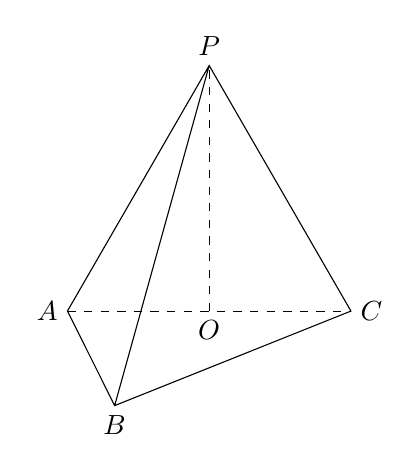
\begin{tikzpicture}[>=latex,scale = 1.8]
\draw (0,0,0) node [left] {$A$} coordinate (A);
\draw (2,0,0) node [right] {$C$} coordinate (C);
\draw (1,0,{sqrt(3)}) node [below] {$B$} coordinate (B);
\draw (1,{sqrt(3)},0) node [above] {$P$} coordinate (P);
\draw (1,0,0) node [below] {$O$} coordinate (O);
\draw (A) -- (B) -- (C) -- (P) -- cycle (P) -- (B);
\draw [dashed] (O) -- (P)  (A) -- (C);
\end{tikzpicture}
\end{center}
(1) 求三棱锥$P-ABC$的体积;\\
(2) 若$M$为$BC$的中点, 求$PM$与平面$PAC$所成角的大小.
\item 已知$f(x)=\log_3(x+a)+\log_3(6-x)$.\\
(1) 若将函数$y=f(x)$的图像向下平移$m$($m>0$)个单位后, 所得的图像经过点$(3,0)$与点$(5,0)$, 求$a$与$m$的值;\\
(2) 若$a>-3$且$a\ne 0$, 解关于$x$的不等式$f(x)\le f(6-x)$.
\item 如图所示的五边形中, $AD=BC=6$, $AB=20$, $\angle ABC=\angle DAB=120^\circ$, $O$为$AB$的中点, 曲线$CMD$上所有点到$O$的距离相等, $MO\perp AB$, $P$为曲线$CM$上的动点, 点$Q$与点$P$关于$OM$对称.
\begin{center}
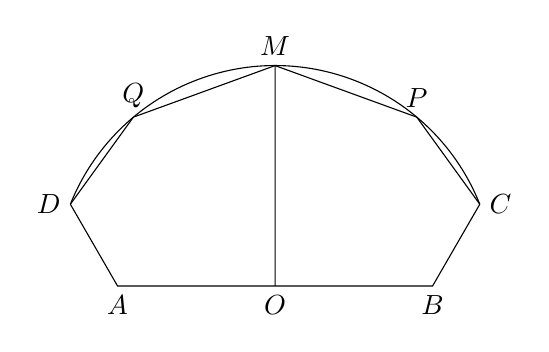
\begin{tikzpicture}[>=latex,scale = 0.2]
\draw (-10,0) node [below] {$A$} coordinate (A);
\draw (10,0) node [below] {$B$} coordinate (B);
\draw (0,0) node [below] {$O$} coordinate (O);
\draw (B) ++ (60:6) node [right] {$C$} coordinate (C);
\draw (A) ++ (120:6) node [left] {$D$} coordinate (D);
\draw (C) arc ({atan(3*sqrt(3)/13)}:{180-atan(3*sqrt(3)/13)}:14);
\draw (0,14) node [above] {$M$} coordinate (M);
\draw (D) -- (A) -- (B) -- (C) (O) -- (M);
\draw (50:14) node [above] {$P$} coordinate (P);
\draw (130:14) node [above] {$Q$} coordinate (Q);
\draw (C) -- (P) -- (M) -- (Q) -- (D);
\end{tikzpicture}
\end{center}
(1) 若$P$在点$D$的位置, 求$\angle POB$的大小;\\
(2) 求五边形$MQABP$面积的最大值.
\item 已知椭圆方程$\Gamma: \dfrac{x^2}{a^2}+\dfrac{y^2}{b^2}=1$($a>b>0$)的左、右焦点为$F_1(-\sqrt{2},0)$、$F_2(\sqrt{2},0)$, $A$为椭圆的下顶点, $M$为直线$l:x+y-4\sqrt{2}=0$上一点.\\
(1) 若$a=2$, $AM$的中点在$x$轴上, 求点$M$的坐标;\\
(2) 直线$l$交$y$轴于点$B$, 直线$AM$经过$F_2$, 若$\triangle ABM$有一个内角的余弦值为$\dfrac 35$, 求$b$的值;\\
(3) 若$\Gamma$上存在点$P$到直线$l$的距离为$d$, 且满足$d+|PF_1|+|PF_2|=6$, 当$a$变化时, 求$d$的最小值.
\item 数列$\{a_n\}$中, $a_1=1$, $a_2=3$, 且对任意$n$($n\ge 2$), 都存在$i$($1\le i\le n-1$), 使得$a_{n+1}=2a_n-a_i$.\\
(1) 求$a_4$的所有可能值;\\
(2) 命题$p$: 若$a_1,a_2,a_3,\cdots,a_8$成等差数列, 则$a_9<30$成立. 证明命题$p$为真, 写出命题$p$的逆命题$q$; 若命题$q$为真, 则证明, 若命题$q$为假, 请举出反例;\\
(3) 对任意正整数$m$, $a_{2m}=3^m$, 求$\{a_n\}$的通项公式.
\end{enumerate}

\end{document}